% Created 2025-05-28 Wed 21:33
% Intended LaTeX compiler: pdflatex
\documentclass[bigger,aspectratio=169]{beamer}
  \usepackage{caption, subcaption, csquotes, amssymb, xcolor}
\usepackage[english]{babel}
\titlegraphic{\includesvg[height=1cm]{./figs/IE_Unicamp}\hspace*{1.25cm}\includesvg[height=1cm]{./figs/SSSA}\hspace*{1.25cm} \includesvg[height=1cm]{./figs/YSI}}
\AtBeginSection[]{
\begin{frame}{Outline}
\tableofcontents[currentsection]
\end{frame}
}
\usepackage[utf8]{inputenc}
\usepackage[T1]{fontenc}
\usepackage{amsmath}
\usepackage{amsfonts}
\usepackage{amssymb}
\usepackage{multicol}
\usepackage{graphicx}
\usepackage{textpos}
\usepackage{caption}
\usepackage{subfig}
\usepackage{svg}
\usepackage{pgfpages}
\usepackage{epstopdf}
\epstopdfsetup{update} % only regenerate if changed
\DeclareGraphicsRule{.eps}{pdf}{.pdf}{`epstopdf #1}
\usepackage{minted}
\usepackage{tikz}
\usetikzlibrary{arrows.meta, positioning, shapes}
\usetheme{Pittsburgh}
\usecolortheme{beaver}
\author{Gabriel Petrini}
\date{July, 2025}
\title{Coding session}
\subtitle{Nelson and Winter (1982) Dynamic competition and technological progress}
\usepackage[style=authoryear]{biblatex}
\addbibresource{~/Org/zotero_refs.bib}
\begin{document}

\maketitle
\begin{frame}{Outline}
\tableofcontents
\end{frame}

\section{Introduction}
\label{sec:org67fa2fa}

\begin{frame}[label={sec:org552cf5e}]{Objectives}
In all blocks, we will

\begin{enumerate}
\item Understand the overall structure of \textcite{dosi_2017_footprint}  model
\item Understand how LSD works
\item Implement the theoretical model on LSD
\item Analyse the model results on LSD
\end{enumerate}
\end{frame}
\begin{frame}[label={sec:orga1b0e06}]{Structure of the sessions}
\begin{description}
\item[{Session 1}] Presents the general structure of the model and of LSD
\item[{Session 2}] Write model equations on LSD
\item[{Session 3}] Analysis of results
\end{description}
\end{frame}
\begin{frame}[label={sec:orgdda7615},fragile]{Repository structure}
 This presentation can be found on this (LINK) repository. In addition:

\begin{description}
\item[{Final.cpp}] Complete equation file for reference
\item[{Coding.cpp}] Script to start with for LSD coding
\item[{Coding.lsd}] Model structure file
\item[{Coding.sa}] Sensitvity Analysis file
\item[{Coding.R}] R script for generating plots
\end{description}

\alert{Important:} Clone this folder under \texttt{LSD/Work/SummerSchool/}
\begin{block}{Missed something?}
\texttt{Final.cpp} contains the complete equation file for reference.
\end{block}
\end{frame}
\section{Session 1}
\label{sec:org94ce79e}
\begin{frame}[label={sec:orge7649e0}]{The Industry model}
\textcite{dosi_2017_footprint} design objective: simplest industrial dynamics model capturing most \alert{stylized facts}:
\begin{itemize}
\item Persistent heterogeneity in productivity and all other performance variables
\item Persistent market share and entry-exit turbulence
\item Skewed size distributions
\item Fat-tailed distribution of growth rates
\item Scaling of the growth-variance relationship
\end{itemize}
\end{frame}
\begin{frame}[label={sec:org4b0a484}]{Equations}
\[ \begin{array}{lrl}
\mbox{Idiosyncratic learning process:} & a_{i,t} = &a_{i,t-1}\cdot (1 + \theta_{i,t})\\
\mbox{Learning shocks} & \theta_{i,t} \sim  & Beta(\beta_1, \beta_2)\\
\mbox{Market selection} & s_{i,t} =  & s_{i,t-1} \cdot \left( 1 + A\cdot\frac{a_{i,t} - \bar{a}_{t}}{\bar{a}_{t}}\right) \\
\mbox{Average productivity} & \bar{a}_{t} =  & \sum_{i=1}^{NF} s_{i, t-1}\cdot a_{i,t} \\
\mbox{Exit condition} & s_{i,t} < & s_{min}\\
\mbox{Entrant productivity} & a_{j,t} =&  \bar{a}_{t}\cdot (1 + \theta_{i,t})\\
\mbox{Entrant market-share} & s_{j,t} =& 1/NF \\
\mbox{Market concentration index} & HHI_{t} =& \sum_{i=1}^{NF} (s_{i})^2 \\
\mbox{Market-share adjustment} &  s_{i} \mapsto & s_{i}\cdot \frac{1}{\sum_{i=1}^{NF} s_{i}} \Rightarrow \sum_{i=1}^{NF} s_{i} = 1 \\
\mbox{Fixed number of firms} & \#\{1, \ldots, n\} =& NF
\end{array}\]
\end{frame}
\begin{frame}[label={sec:orgada5e67}]{DAG of industry model}
\resizebox{\linewidth}{!}{%
  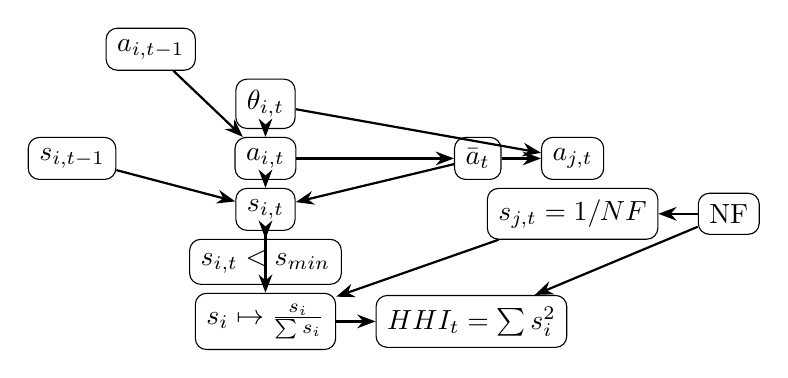
\begin{tikzpicture}[
    node distance=.1cm and 0.5cm,
    every node/.style={draw, rounded corners, minimum height=1.2em, inner sep=4pt, align=center},
    arrow/.style={-{Stealth}, thick}
    ]

    % Nodes
    \node (theta)        {$\theta_{i,t}$};
    \node (ai_tm1)       [above left=of theta] {$a_{i,t-1}$};
    \node (ai_t)         [below=of theta] {$a_{i,t}$};
    \node (si_tm1)       [left=1.5cm of ai_t] {$s_{i,t-1}$};
    \node (abar_t)       [right=2cm of ai_t] {$\bar{a}_t$};
    \node (si_t)         [below=of ai_t] {$s_{i,t}$};
    \node (exit)         [below=of si_t] {$s_{i,t} < s_{min}$};

    \node (aj_t)         [right=of abar_t] {$a_{j,t}$};
    \node (sj_t)         [below=of aj_t] {$s_{j,t} = 1/NF$};

    \node (norm_s)       [below=of exit] {$s_i \mapsto \frac{s_i}{\sum s_i}$};
    \node (HHI_t)        [right=of norm_s] {$HHI_t = \sum s_i^2$};

    \node (NF)           [right=of sj_t] {NF};

    % Arrows
    \draw[arrow] (ai_tm1) -- (ai_t);
    \draw[arrow] (theta) -- (ai_t);
    \draw[arrow] (ai_t) -- (abar_t);
    \draw[arrow] (si_tm1) -- (si_t);
    \draw[arrow] (ai_t) -- (si_t);
    \draw[arrow] (abar_t) -- (si_t);
    \draw[arrow] (si_t) -- (exit);

    \draw[arrow] (abar_t) -- (aj_t);
    \draw[arrow] (theta) -- (aj_t);
    \draw[arrow] (NF) -- (sj_t);
    \draw[arrow] (NF) -- (HHI_t);
    \draw[arrow] (si_t) -- (norm_s);
    \draw[arrow] (sj_t) -- (norm_s);
    \draw[arrow] (norm_s) -- (HHI_t);

    % Optional: Labels or braces could be added if needed
  \end{tikzpicture}
}
\end{frame}
\begin{frame}[label={sec:org63baa29},fragile]{Sequence of events}
 At time \(t = 0\), there are \(NF\) identical incumbent firms with equal \(a_{i,t=0}\) and \(s_{i,0}\).
At each time step \(t = 1, 2, \ldots, T\):
\begin{enumerate}
\item Firms learn (updates (\(a_{i}\))
\item Firms computes market share (updates \(s_{i}\))
\item Market concentration index (\(HHI\)) is computed
\item Firms exits the market if \(s_{i} < s_{min}\)
\item Firms enter to keep \(NF\) firms in the market
\item Incumbents variables (\(a_{j}\), \(s_{j}\)) are set
\item Market shares are re-scaled proportionally to ensure \(\sum s_{i} = 1\)
\end{enumerate}
\begin{block}{Model logical order (later)}
The exit-entry process is time-coordinated during each simulated time step by the technical variable \texttt{exit\_entry}: \texttt{HHI} > \texttt{exit\_decision} > \texttt{s} rescaling
\end{block}
\end{frame}
\begin{frame}[label={sec:orge0aa4c6}]{Parameters and initial values}
\begin{table}[htbp]
\caption{Baseline parameters}
\centering
\begin{tabular}{ccc}
\hline
 & Desc & Value\\
\hline
\(\eta\) & Innovation opportunity support & 0.3\\
\(\beta_{1}, \beta_{2}\) & beta distribution parameters & 1.0; 5.0\\
\(A\) & replicator dynamics intensity & 1\\
\(s_{min}\) & minimum market share to not exit & 0.01\\
\(NF\) & number of firms & 10\\
\hline
\(a_{i}_{}\) & Initial Firm-level productivity & 1.0\\
\(s_{i}\) & Initial Firm market-share & \(1/NF\)\\
\hline
\end{tabular}
\end{table}
\end{frame}
\begin{frame}[label={sec:org6de0f90},fragile]{Model structure and data organization I}
 Besides the equation files (\texttt{.cpp} or \texttt{.h}), LSD defines the model structures on a different file (extension \texttt{.lsd}).
This special file has:

\begin{itemize}
\item Variables and parameters names
\item Model structure (where elements are)
\item Initial and parameter values
\item Simulation settings
\item Number of objects
\item Variables to plot, analyse, debug, etc
\end{itemize}
\begin{block}{LSD and OOP}
This structure ensure the modeler to think in terms of data structure.
\end{block}
\end{frame}
\begin{frame}[label={sec:org08d7821}]{Model structure and data organization II}
\begin{figure}[htbp]
\centering
\includegraphics[clip,trim=0 0 0 0,width=.8\textwidth,height=.75\textheight]{figs/Structure_Industry_LSD.png}
\caption{Structure of industry model}
\end{figure}
\end{frame}
\section{Session 2}
\label{sec:orgab5fb40}

\begin{frame}[label={sec:orgb9d624d}]{Where we are and to where we go?}
\end{frame}

\begin{frame}[label={sec:org0040fb1},fragile]{C++ for LSD I}
 LSD adds macros to \texttt{C++}.
As a consequence, some basic knowledge on \texttt{C++} is usefull.
What we need to know here?
\begin{columns}
\begin{column}{0.4\columnwidth}
\begin{block}{In python}
\begin{verbatim}
x = 5 # A comment
y = 2.5
## We do not need to
## look at pointers
\end{verbatim}
\end{block}
\end{column}
\begin{column}{0.4\columnwidth}
\begin{block}{In C++}
\begin{verbatim}
int x = 5; // A comment
double y = 2.5;
object *agent; // Latter
\end{verbatim}
\end{block}
\end{column}
\end{columns}
\begin{block}{Compilation}
Different from python and R, we need to \alert{compile} our code before using it.
\end{block}
\end{frame}
\begin{frame}[label={sec:org2a3cbc0},fragile]{C++ for LSD II}
 To avoid initializing everything, LSD has some already initialized variables:

\begin{verbatim}
v[0] = 10; // We can assing number to
v[1] = 50; // a vector (always available)
T; // Current simulation time
i = 1; // i,h,j,k can be used for integers
cur; cur1; // Pre-allocated pointers
\end{verbatim}

Those are \alert{local variables} that we can use on equations.
\begin{block}{Debbuging}
LSD has an internal debbuger that allow us to look to local variables on the fly.
\end{block}
\end{frame}
\begin{frame}[label={sec:org2c3d4e2},fragile]{Macros I}
 \begin{figure}[htbp]
\centering
\includegraphics[width=.9\linewidth]{./figs/Macros_LSD.pdf}
\caption{\label{}General structure of most LSD macros}
\end{figure}

Examples:
\begin{description}
\item[{VLS(POS, ``NAME'', 1)}] Returns the value of variable \texttt{NAME} at lag \texttt{1} at position \texttt{POS}
\item[{SUMS(POS, ``NAME'')}] Sums the value of variable \texttt{NAME} at position \texttt{POS}
\item[{SEARCHS(PARENT, ``AGT'')}] Searches for agent \texttt{AGT} starting from \texttt{PARENT}
\item[{WRITES(POS, ``NAME'', 1)}] Overwrites variable \texttt{NAME} at lag \texttt{1} at position \texttt{POS}
\end{description}
\end{frame}
\begin{frame}[label={sec:org27be82f}]{Macros II}
\begin{figure}[htbp]
\centering
\includegraphics[width=.9\linewidth]{figs/LSD_Macros_ScreenShot.png}
\caption{Other LSD macros}
\end{figure}
\end{frame}
\begin{frame}[label={sec:org89db4f9},fragile]{Simple example I}
 How can we write the following equation using LSD syntax?

\[X_{t} = X_{t-1} + m\]

\begin{verbatim}
EQUATION("X") // This is a one line comment
/*
This is a long comment
*/
v[0] = VL("X",1); //past value of X, lagged of 1 period
v[1] = V("m"); //current value of m (variable or parameter)
v[2] = v[0] + v[1]; // v[n] are local variables
RESULT(v[2]) // Specify the output of the function
\end{verbatim}
\begin{block}{Variable or parameter?}
As a rule of thumb, variables have an \texttt{EQUATION} associated, parameters do not.
\end{block}
\end{frame}
\begin{frame}[label={sec:orga1e118b},fragile]{Simple example II}
 How can we write the following equation using LSD syntax?

\[Y_{t} = \sum_{i=1}^{n} X_{n,t} + W_{n,t}\]


\begin{verbatim}
EQUATION("Y")
v[0] = 0; // Initialize the Accumulation
CYCLE(cur, "Firm") { // Similar to a for-loop in other languages
    v[1] = VS(cur, "X"); // cur points to a "Firm" object
    v[2] = VS(cur, "W"); // cur is a locally defined pointer
    v[3] = v[1] + v[2];
    v[0] = v[0] + v[3];
}
RESULT(v[0])
\end{verbatim}
\end{frame}
\begin{frame}[label={sec:org94d33d3},fragile]{Equation file}
 Any equation file (\texttt{.cpp}) must contain the following text:
\begin{verbatim}
// File created using org-mode tangle feature.
#include "fun_head.h" // This is mandatory

MODELBEGIN

// Your code goes here

MODELEND
void close_sim(void) {}
\end{verbatim}

In our session, we will copy-and-paste the initialization equation and continue from there.
\end{frame}
\begin{frame}[label={sec:org459268b},fragile]{Other files}
 Besides the equation files (\texttt{.cpp} or \texttt{.h}), LSD defines the model structures on a different file (extension \texttt{.lsd}).
This special file has:

\begin{itemize}
\item Variables and parameters names
\item Model structure (where elements are)
\item Initial and parameter values
\item Simulation settings
\item Number of objects
\item Variables to plot, analyse, debug, etc
\end{itemize}
\begin{block}{LSD and OOP}
This structure ensure the modeler to think in terms of data structure.
\end{block}
\end{frame}
\begin{frame}[label={sec:org61ea3c7}]{Structure of NW model}
\begin{center}
\includegraphics[width=.9\linewidth]{figs/NW_Structure.png}
\end{center}
\end{frame}
\begin{frame}[label={sec:orgc44611a}]{Simulation pipeline}
Whenever running a model on LSD, we need to:

\begin{enumerate}
\item Design a model (on paper);
\item Write the code implementing the equation;
\item Define the model structure and initialization;
\item Run the simulation;
\item Analyse the results.
\end{enumerate}
\end{frame}
\begin{frame}[label={sec:org5ee693b}]{Memo: Equations}
\[ \begin{array}{lrl}
\mbox{Idiosyncratic learning process:} & a_{i,t} = &a_{i,t-1}\cdot (1 + \theta_{i,t})\\
\mbox{Learning shocks} & \theta_{i,t} \sim  & Beta(\beta_1, \beta_2)\\
\mbox{Market selection} & s_{i,t} =  & s_{i,t-1} \cdot \left( 1 + A\cdot\frac{a_{i,t} - \bar{a}_{t}}{\bar{a}_{t}}\right) \\
\mbox{Average productivity} & \bar{a}_{t} =  & \sum_{i=1}^{NF} s_{i, t-1}\cdot a_{i,t} \\
\mbox{Exit condition} & s_{i,t} < & s_{min}\\
\mbox{Entrant productivity} & a_{j,t} =&  \bar{a}_{t}\cdot (1 + \theta_{i,t})\\
\mbox{Entrant market-share} & s_{j,t} =& 1/NF \\
\mbox{Market concentration index} & HHI_{t} =& \sum_{i=1}^{NF} (s_{i})^2 \\
\mbox{Market-share adjustment} &  s_{i} \mapsto & s_{i}\cdot \frac{1}{\sum_{i=1}^{NF} s_{i}} \Rightarrow \sum_{i=1}^{NF} s_{i} = 1 \\
\mbox{Fixed number of firms} & \#\{1, \ldots, n\} =& NF
\end{array}\]
\end{frame}
\begin{frame}[label={sec:org8eda071},fragile]{Firm-level productivity (\(a_{i}\)\textsubscript{nil})}
 \begin{equation}
a_{i,t} = a_{i,t-1}\cdot (1 + \theta_{i,t})
\end{equation}

\begin{verbatim}
EQUATION("a")
// Firm knowledge/productivity
v[0] = CURRENT;
v[1] = V("eta");
v[2] = V("beta1");
v[3] = V("beta2");
v[4] = beta(v[2], v[3]);
v[5] = v[0] * (1 + v[1] * v[4]);
RESULT(v[5])
\end{verbatim}
\end{frame}
\begin{frame}[label={sec:orgd78fa78},fragile]{Market-share (\(s_{i}\))}
 \begin{equation}
s_{i,t} = s_{i,t-1} \cdot \left( 1 + A\cdot\frac{a_{i,t} - \bar{a}_{t}}{\bar{a}_{t}}\right)
\end{equation}


\begin{verbatim}
EQUATION("s")
// Firm size/market share
v[0] = CURRENT;
v[1] = V("A");
v[2] = V("a");
v[3] = V("aAvg");
v[4] = (v[2] - v[3])/v[3];
v[5] = v[0] * (1 + v[1] * v[4]);
RESULT(v[5])
\end{verbatim}
\end{frame}
\begin{frame}[label={sec:org3c3203a},fragile]{Exit condition}
 \begin{verbatim}
EQUATION("exit_decision")

v[0] = V("s"); v[1] = V("sMin");
// update entrant firm productivity and market share
if (v[0] < v[1]) {
  v[2] = V("eta"); v[3] = V("beta1"); v[4] = V("beta2");
  v[5] = beta(v[3], v[4]);
  v[6] = V("aAvg");
  v[7] = v[6] * (1 + v[2] * v[5]);
  WRITE( "a", v[7] );
  WRITE( "s", 1 / COUNT( "Firm" ) );
}
RESULT(0)
\end{verbatim}
\end{frame}
\begin{frame}[label={sec:org707f1d1},fragile]{Market-level Productivity (Weighted) Average (\(\bar{a_{t}}\))}
 \begin{equation}
\bar{a}_{t} =  \sum_{i=1}^{NF} s_{i, t-1}\cdot a_{i,t}
\end{equation}


\begin{verbatim}
EQUATION( "aAvg" )
// Mean knowledge/productivity

v[0] = 0;        // accumulator
CYCLE(cur, "Firm") {
  v[1] = VLS( cur, "s", 1 );
  v[2] = VS( cur, "a" );
  v[3] = v[1] * v[2];
  v[0] += v[3] ;
}
RESULT( v[0] )
\end{verbatim}
\end{frame}
\begin{frame}[label={sec:org9008db5},fragile]{Entry-Exit condition}
 \begin{verbatim}
EQUATION( "exit_entry" )
// Trigger market-wise exit-entry dynamics and re-scale shares
V( "HHI" ); // first, compute HH index before exits

// second, ensure firms have decided on exit
CYCLE(cur, "Firm") {VS( cur, "exit_decision" );}

v[0] = 1 / SUM( "s" ); // factor to scale back to sum = 1
CYCLE(cur, "Firm") { // third, rescale market shares after exits
  v[1] = VS( cur, "s" );
  v[2] = v[0] * v[1];
  WRITES( cur, "s", v[2]);
}
RESULT( SUM("s") )
\end{verbatim}
\end{frame}
\begin{frame}[label={sec:org4a2badb},fragile]{Herfindahl-Hirschman concentration index (\(HHI\))}
 \begin{equation}
HHI_{t} = \sum_{i=1}^{NF} (s_{i})^2
\end{equation}


\begin{verbatim}
EQUATION( "HHI" )
// Herfindahl-Hirschman concentration index
v[0] = WHTAVE( "s", "s" );
RESULT( v[0] )
\end{verbatim}
\begin{block}{Note on WHTAVE(LS)}
\texttt{WHTAVE} (weighed average, not used here in the strict sense) computes the sum of \(s\times s\) over every firm
\end{block}
\end{frame}
\begin{frame}[label={sec:org7c1c948},fragile]{Initialization I}
 Firm-level initialization can be set for every \(NF\) objects on the LSD browser.
The same applies for every other initial condition.

On the following slide, we will see an alternative way in which we control some few parameters and create \(NF-1\) copies of a example object.

\begin{verbatim}
ADDNOBJ_EX("TypeOfAgent", number, *pointer);
\end{verbatim}
\begin{block}{Semi-automatic initialization and sensitivity analysis}
By doing this, we automate the model initialization to test different model configurations (next lecture)
\end{block}
\end{frame}
\begin{frame}[label={sec:org2089fd5},fragile]{Initialization II}
 \begin{verbatim}
EQUATION( "init" )
PARAMETER;                  // turn into parameter (run once)
// finds the agent on memory
cur = SEARCH( "Market" ); cur1 = SEARCHS(cur, "Firm" );

v[0] = V("A0"); // We define
v[1] = V("Nfirm"); // We define
v[2] = 1 / v[1]; // Fair share
// Overwrites the lag 1 of "a" to v[0] at time 1
WRITELLS(cur1, "a", v[0], 1, 1);
WRITELLS(cur1, "s", v[2], 1, 1);
// Adds N - 1 copies of cur1 agent located under cur
ADDNOBJ_EXS(cur, "Firm", v[1] - 1, cur1);
RESULT( 1 )
\end{verbatim}
\end{frame}
\section{Session 3}
\label{sec:orgec1dc36}

\begin{frame}[label={sec:org5c2dc09}]{Where we are and to where we go?}
\end{frame}

\begin{frame}[label={sec:orged35054}]{Required packages}
\end{frame}

\begin{frame}[label={sec:orgc36da0d}]{Required files}
\end{frame}
\end{document}
